\documentclass{article}
\usepackage{graphicx}
\usepackage{float}
\bibliographystyle{unsrt}

\title{CMSC 6950 Final Project - argopy}
\author{Michael King}

\begin{document}
\maketitle

\section{Introduction}

The objective of this project was to select an open source software package and perform computational tasks using data obtained from a package of choice. The scientific package chosen for my project is called argopy \cite{maze2020argopy}. argopy is a Python library that can be used to download, analyze and interpret ocean data collected by Argo floats. In particular, the argopy Python library permits users to obtain Argo float measurements from Argo floats worldwide that measure pressure, temperature and salinity of the worlds oceans from the surface to 2000m depth every 10 days. Traditionally, the large number of files, data variables and use of jargon associated with the Argo data often accompanied a challenging workflow, especially for new users. The motivation of argopy was to provide a Python friendly library where Argo float data can be easily accessible and readable for users who are new to and/or experts with Argo float data. For this project, two computational tasks have been carried out using data extracted from the argopy Python library and other Python modules such as numpy, pandas, geopandas and matplotlib. 

    

\section{Results}

Herein, the results for each computational task will be presented. The first computational task will focus on visualizing the position of Argo floats in a region southeast of Florida, USA,  and how the total number of floats changes each year. The second computational task is used to visualize the trajectory and temperature variation of two Argo floats with time since the float's deployment.

\subsection{Task 1- Total Argo float numbers through time}

The objective for my first computational task was to retrieve Argo float data collected from 2001 to 2006 using argopy and then use this data to visualize the change in the total number of Argo floats per year within a region of the Atlantic Ocean, southeast of Florida, USA. This task began by using the ArgoDataFetcher to download Argo data within user specified coordinates for a specified time frame (2001-01-01 to 2006-12-31). Following this step, the downloaded Argo data (stored as an xarray.Dataset) was converted into a Pandas dataframe to investigate the contents of the data before being exported as a csv file. This csv file served as the intermediate data file used to perform my first computational task. Next, this csv file was loaded into a new python script as a Pandas dataframe in order to begin the final data filtering and sorting steps. First, using the Pandas functionality on the 'TIME' column for the Argo dataset, a column of years was added that represented the year the Argo data was collected. This step was carried out in order to plot the data by year in the final steps of this computational task. Next, prior to defining the Python code used for plotting, the Pandas dataframe was then split into 6 different dataframes so that each dataframe only contained Argo data from a certain year from 2001 to 2006. Subsequently, each dataframe containing Argo float data from 2001 to 2006 was then appended to the dataframe of its subsequent year in order to calculate the total number of Argo floats present each year. For example, the dataframe for Argo floats deployed in 2002 (400) was appended to the total in 2001 (33) in order to create a dataframe with the total number of Argo floats over those two years (433). Following the completion of these data filtering steps, all 6 dataframes were exported as csv files so that they could be then imported into another Python script used to create the visualization for task 1. For plotting and visualizing the data, the matplotlib and geopandas Python libraries were used to plot the position and total number of Argo floats per year (Figure \ref{fig:task 1}). Each plot included a base map of North America (extracted using a dataframe obtained from geopandas) in order to provide a clearer spatial reference of the Argo float locations.

\begin{figure}[H]
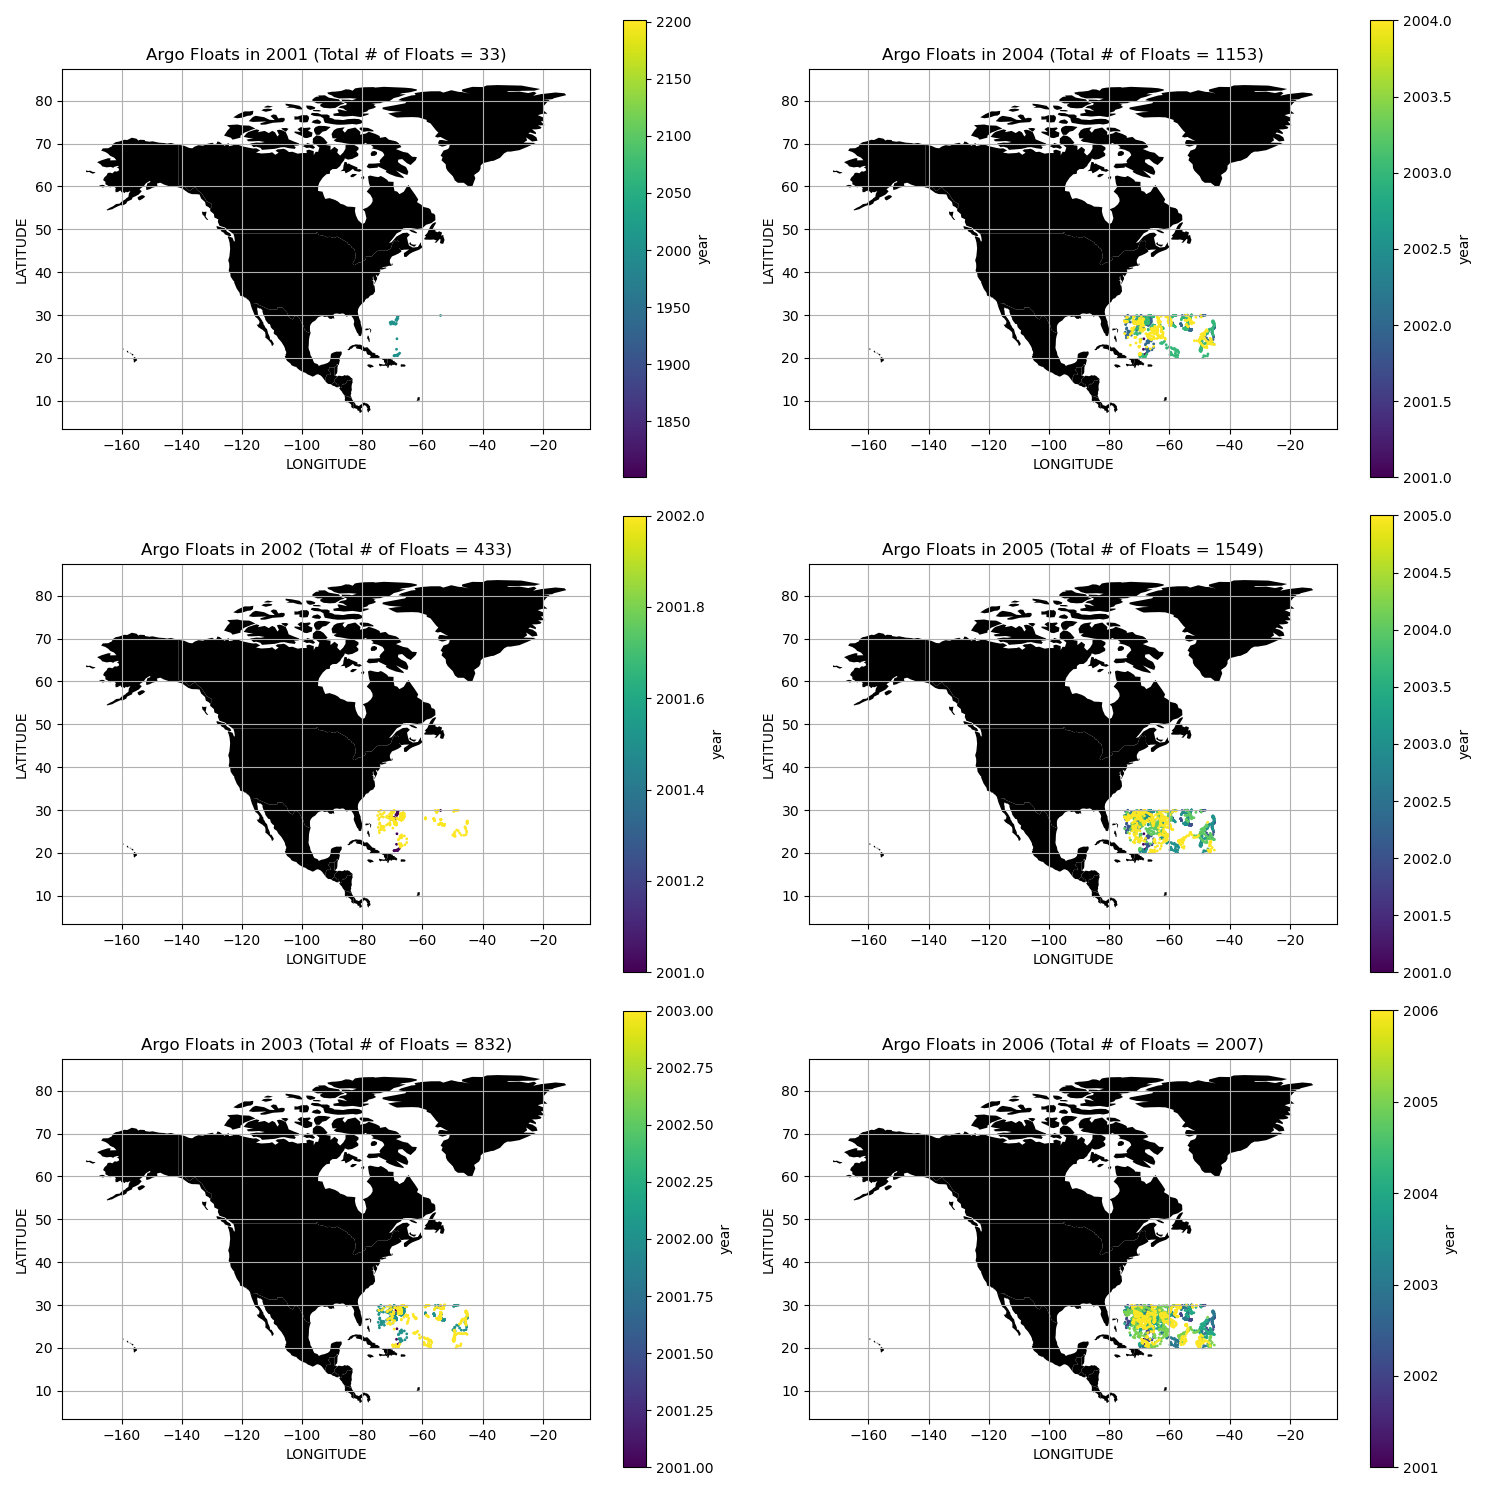
\includegraphics[width=\textwidth,height=\textheight,keepaspectratio]{total_argo.png}
\caption{Total number of Argo floats for each year from 2001 to 2006 in a region southeast of Florida, USA.}
\label{fig:task 1}
 
\end{figure}


\subsection{Task 2 - Argo float trajectories}

The objective of my second computational task was to visualize the trajectory of two Argo floats and their temperature variations since deployment. To do this, data from two Argo floats were extracted using the ArgoDataFetcher function in argopy. The specific Argo floats chosen for this computational task were selected by examining the distribution of Argo floats within the Atlantic Ocean using the argopy.dashboard() in Jupyter notebook. This command allows one to visualize all Argo floats in an interactive interface that contains detailed information for each Argo float. Following the extraction of Argo data using argopy, the data was converted into a pandas dataframe and extracted as a csv file that served as the intermediate file for this computational task. This csv file was then loaded into a new python script that was used for additional data sorting. Prior to plotting the Argo data, the data was split into two different dataframes based on the platform number of the two Argo floats (Argos 6902754 and 6902696) and exported as csv files. Following this step, a new python script used for plotting was created to make two scatter plots (each showing the trajectory and cycle numbers of a particular Argo float) and 4 additional graphs displaying the temporal evolution of latitude, cycle number, longitude, and temperature since the deployment of each Argo float (Figure \ref{fig:task 2}). For the two scatter plots showing the trajectory of each Argo float with cycle number, a base map of Canada was added using a geopandas dataframe in order to provide spatial reference of the Argo float positions with respect to Canada.

\begin{figure}[H]
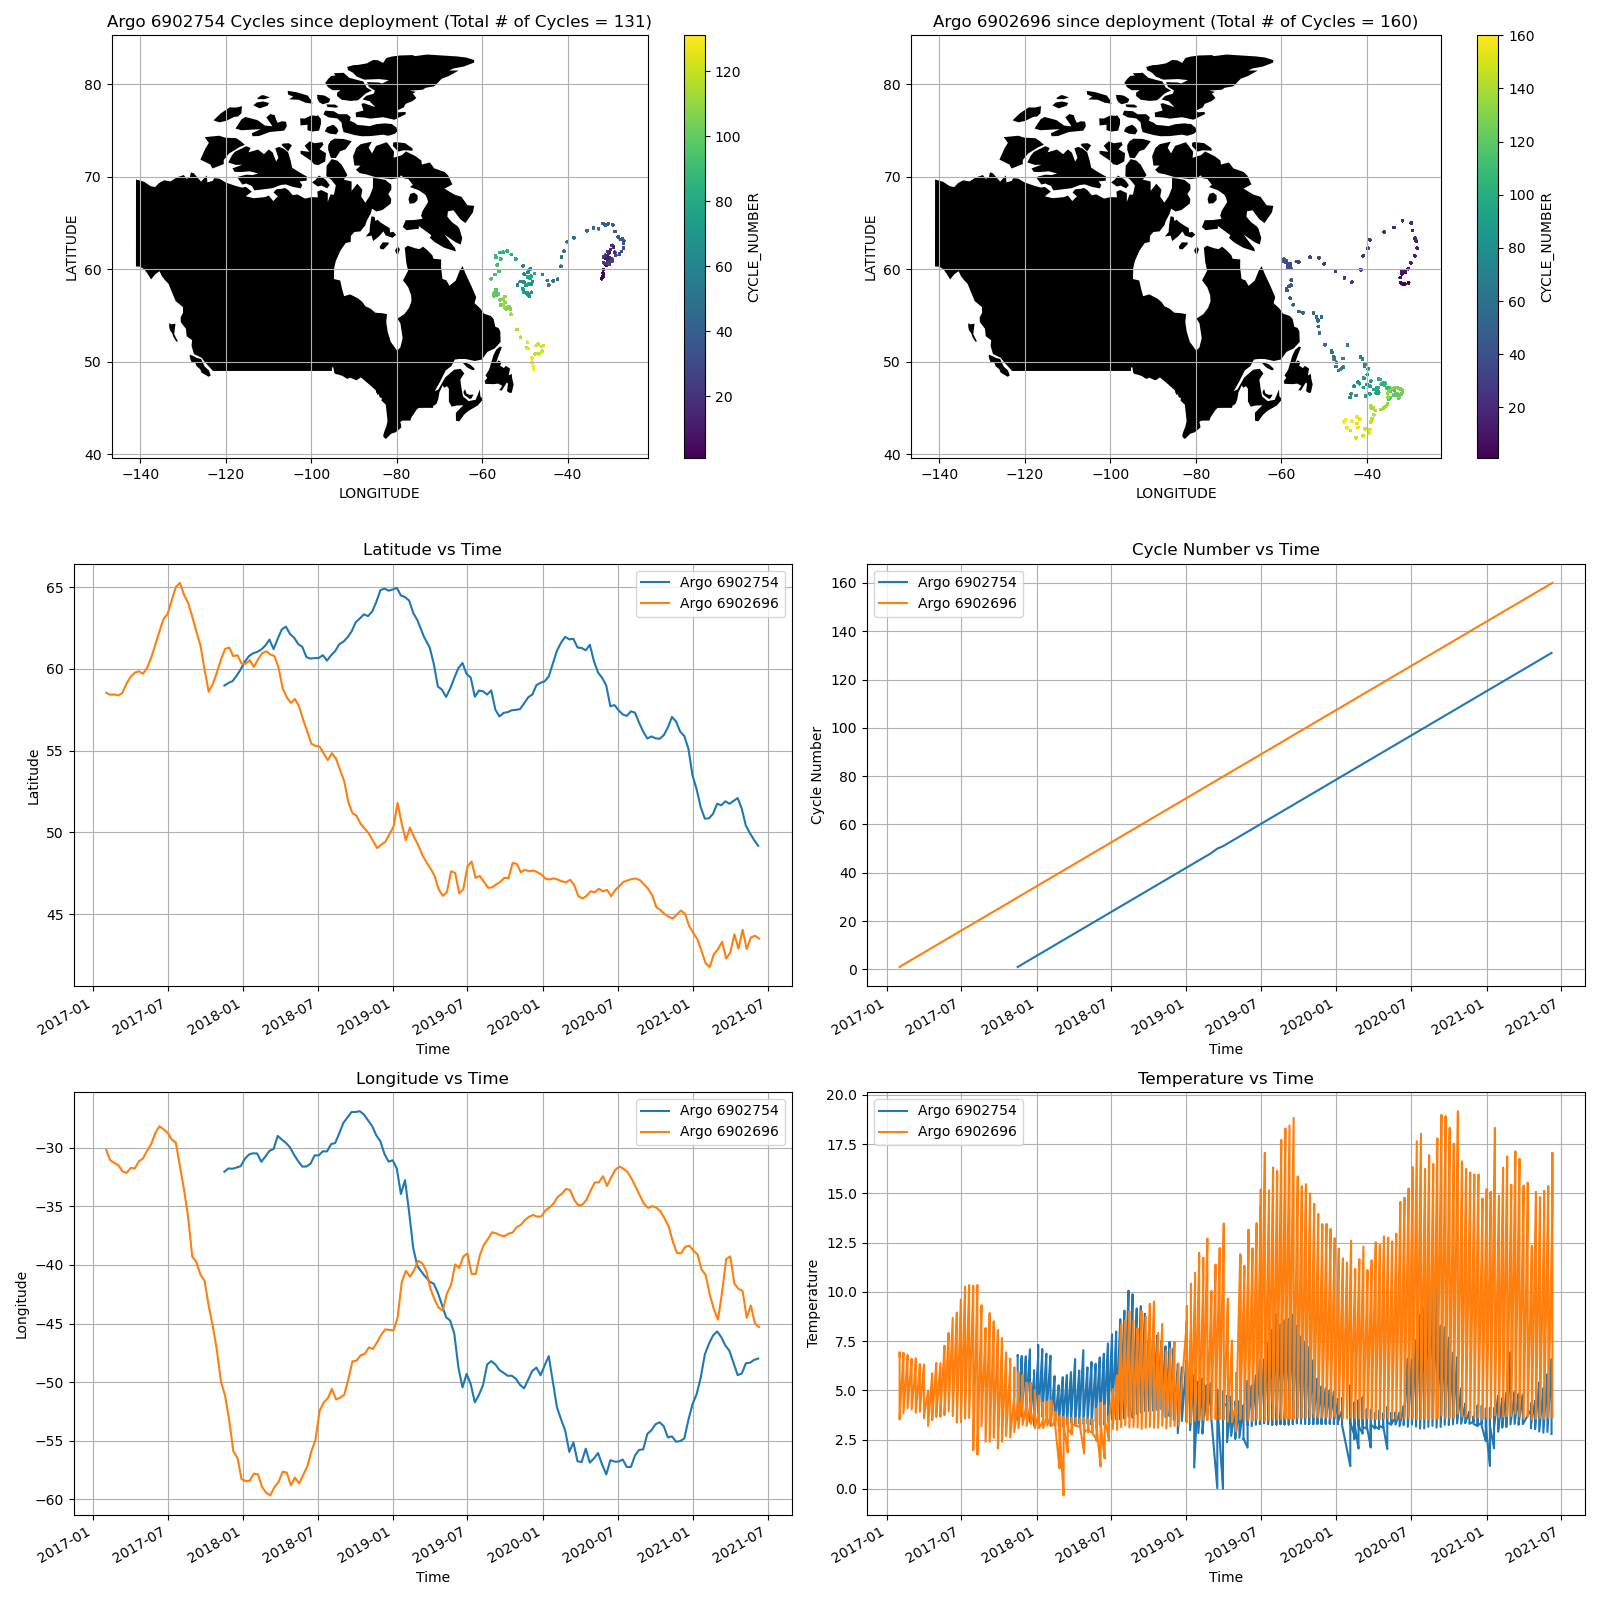
\includegraphics[width=\textwidth,height=\textheight,keepaspectratio]{argo_trajectory.png}
\caption{Trajectory and temperature variation with time of two Argo floats located within the Atlantic Ocean, offshore Newfoundland and Labrador.}
\label{fig:task 2}
\end{figure}
 
 

\section{Conclusions}

In conclusion, two computational tasks were performed using data extracted from the argopy Python library. The first computational task provided a visualization of total Argo float numbers through time using the pandas, matplotlib and geopandas Python libraries. The second computational task consisted of extracting data from two Argo floats using argopy. The trajectory and temperature variation with time was then visualized by also using the pandas, matplotlib and geopandas Python libraries.

\bibliography{refs}

\end{document}